\documentclass[tcc]{ic}

%%%%%%%%%%%%%%%%%%%%%%%%%%%%%%%%%%%%
\hypersetup{
colorlinks = {true},
linktocpage = {false},
plainpages = {false},
linkcolor = {Blue},
citecolor = {Blue},
urlcolor = {Red},
unicode = {true},
pdftitle = {titulo}, 
pdfauthor = {autor},
pdfsubject = {Trabalho de Conclusão de Curso},
pdfkeywords={palavras-chave},
pdfcreator = {LaTeX2e},
pdffitwindow = {false},
pdfstartview = {FitH},
pdftoolbar = {true},
pdfpagemode = {UseOutlines},
pdfview = {XYZ null null null}
}
%%%%%%%%%%%%%%%%%%%%%%%%%%%%%%%%%%%%%
\graphicspath{ {./images/} }
\usepackage{lettrine}
\usepackage{smartdiagram}
\usepackage{lscape}
\usepackage{longtable}
\usepackage{dsfont}
\usepackage{comment}
\usepackage[utf8]{inputenc}
\inputencoding{latin1}
\inputencoding{utf8}
\usepackage{amstext}
\usepackage{subfigure}
\usepackage[colorinlistoftodos,prependcaption]{todonotes}


\usepackage{chngcntr}
\counterwithout{table}{chapter}
\counterwithout{figure}{chapter}
\counterwithout{equation}{chapter}
\usepackage{amsmath}
\usepackage{amsfonts}
\usepackage{amssymb}


\titulo{Modelagem Dinâmica e Estática do Braço Robótico UR5}

\autor{Valdir de Souza Junior}{vsj@ic.ufal.br}{}

\orientador{Prof. Dr. Erick de Andrade Barboza}{Instituto de Computação}{Universidade Federal de Alagoas}

\examinador{avaliador}{}{Instituto de Computação}{Universidade Federal de Alagoas}

\examinadorTres{avaliador2}{}{Instituto de Computação}{Universidade Federal de Alagoas}

\dataMesAno{Dezembro}{2020}

\begin{document}

\selectlanguage{portuguese}

\capa

\begin{agradecimentos}




\vspace{2em}
\begin{flushright}
autor
\end{flushright}


\vspace{30em}
\begin{epigraph}{segundo nome, \textit{primeiro nome}}
``frase''
\end{epigraph}



\end{agradecimentos}

\begin{resumo}

resumo

\vspace{1em}
\textbf{Palavras-chave}: 
\end{resumo}

\begin{abstract}
abstract

\end{abstract}
\vspace{1em}
\textbf{Key-words}:  A, B, C

%\end{abstract}

% Figuras
\makefigurespage

% Tabelas
\maketablespage
\listoftables

% Algoritmos
\listofalgorithms

% Abreviaturas (devem estar em ordem alfabética)
\makeabrevpage{\item [IC] Instituto de Computação}

% Símbolos (devem estar em ordem alfabética)
\makesymbolspage{\item [IC] Instituto de Computação
}

\tableofcontents

\inicio



\mychapter{Introdução}{cap:introducao} \lhead{INTRODUÇÃO}

TODO
\mychapter{Fundamentação Teórica}{cap:fundamentacao-teorica} \lhead{Fundamentação Teórica}
\mychapter{Fundamentação Teórica}{cap:fundamentacao-teorica} \lhead{Fundamentação Teórica}
\mychapter{Fundamentação Teórica}{cap:fundamentacao-teorica} \lhead{Fundamentação Teórica}
\include{capitulos/fundamentacao}
TODO2
\mychapter{Materiais e Métodos}{cap:materiais-metodos} \lhead{Materiais e Métodos}
\mychapter{Materiais e Métodos}{cap:materiais-metodos} \lhead{Materiais e Métodos}
\mychapter{Materiais e Métodos}{cap:materiais-metodos} \lhead{Materiais e Métodos}
\include{capitulos/materiais}
TODO
\mychapter{Resultados e Discussões}{cap:resultados} \lhead{Resultados}


\section{Tabela de Denavit-Hartenberg}


\begin{table}[ht]
\centering
\begin{tabular}[t]{lcccc}
\toprule
 &$q_i [rad]$ &$d_i [m]$ &$a_i [m]$ &$\alpha_i [rad]$\\
\midrule
Junta 1& $q_1$& 0.089159&0&$\frac{\pi}{2}$\\
Junta 2& $q_2$& 0 &-0.425&0\\
Junta 3& $q_3$& 0 &-0.39225&0\\
Junta 4& $q_4$& 0.10915 &0&$\frac{\pi}{2}$\\
Junta 5& $q_5$& 0.09465 &0&-$\frac{\pi}{2}$\\
Junta 6& $q_6$& 0.0823 &0&0\\
\bottomrule
\end{tabular}
\caption{Tabela de Denavit-Hartenberg}
\end{table}%

\section{Justificativa}

TODO
\mychapter{Conclusão}{cap:conclusao}

\begin{equation} \label{threshold:fun}
  \phi(x) =
  \left\{
      \begin{array}{ll}
        1, & \mbox{if } x \geq 0 \\
        0, & \mbox{if } x < 0
      \end{array}
  \right.
\end{equation}
TODO
\mychapter{Temporário}{cap:temporario} \lhead{Temporário}

\section{Justificativa}

O controle de movimentação de robôs é uma competência chave para os fabricantes, e o desenvolvimento atual está focado em aumentar o desempenho do robô, reduzindo custos, melhorando a segurança e introduzindo novas funcionalidades conforme descrito
em \cite{brogaardh2007present}, há necessidade de melhorar continuamente os modelos e métodos 
de controle a fim de cumprir todos os requisitos conflitantes, por exemplo,
maior desempenho para um robô de peso menor e, portanto, menor rigidez mecânica.

O motivo para este tipo de desenvolvimento é, naturalmente, a redução de custos, mas também existem outros benefícios menores como menor consumo de energia, aprimoramento da destreza, melhorias em segurança
e menor impacto ambiental. A necessidade de redução de custos pode resultar no uso
de componentes mais otimizados, de menor valor, que geralmente têm maior variação em seus resultados,
por exemplo, variação da rigidez da caixa de engrenagens ou nos parâmetros que descrevem o
braço mecânico. A redução de custos às vezes também resulta em um nível mais alto de perturbações e
não linearidades em alguns dos componentes, por exemplo, nos atuadores ou nos sensores.

Um robô industrial é uma máquina de uso geral para automação industrial, e apesar de que os requisitos de uma determinada aplicação possam ser formulados com precisão, não há limites para o que os usuários do robô desejam com relação ao desempenho e à funcionalidade desejáveis do controle de movimento de um robô. O controle de movimentação depende da aplicação. Quanto melhor o desempenho,
mais aplicações estarão sujeitas à serem automatizadas por um modelo de robô específico.
Alguns exemplos de requisitos são:

\begin{itemize}
   \item Alta precisão no seguimento de caminho em aplicações contínuas (por exemplo, soldagem a laser, corte a laser, corte com jato de água).
   \item Precisão de alta velocidade em aplicações contínuas (por exemplo, pintura ou dispensação).
   \item Baixo tempo de ciclo (alta velocidade e aceleração) em aplicações discretas (por exemplo,manuseio de materiais).
   \item Pequenos overshoots e um curto tempo de acomodação em aplicações de processo discretas
(por exemplo, soldagem por pontos).
   \item Alto controle de rigidez em aplicações de contato (por exemplo, usinagem).
 \end{itemize}

Para manipuladores industriais com peso e custo otimizados, os requisitos acima só podem ser manipulado por inteligência computacional aumentada, ou seja, controle de movimento aprimorado. O controle de movimento de robôs manipuladores industriais é um desafio
tarefa, que tem sido estudada por pesquisadores acadêmicos e industriais. Alguns resultados da pesquisa acadêmica foram implementados com sucesso em aplicações industriais reais, enquanto outros resultados estão longe
de ser relevante para a realidade industrial. Até certo ponto, o desenvolvimento de algoritmos de controle de movimento seguiram duas rotas distintas, uma por pesquisadores acadêmicos e outra por fabricantes de robôs.


A situação pode ser parcialmente explicada pelo fato de que os algoritmos de movimento usados na indústria às vezes são considerados segredos comerciais. Devido a difícil situação competitiva entre os fabricantes de robôs, os algoritmos são
raramente publicado. Outra explicação é que os pesquisadores de controle de robôs acadêmicos muitas vezes aplicam matemática avançada em alguns aspectos selecionados de sistemas relativamente pequenos, enquanto os pesquisadores e desenvolvedores de robôs industriais lidam com todos os aspectos significativos de um sistema complexo onde a proposta matemática avançada frequentemente não pode ser aplicada. Além disso, os problemas que
a indústria de robôs às vezes presente pode incluir muitos aspectos de engenharia para ser atraente para a comunidade acadêmica. Pesquisa de robôs industriais e
o desenvolvimento deve equilibrar atividades de curto prazo e atividades de longo prazo. Colaborações de pesquisa a longo prazo entre a indústria e a academia devem ser possíveis, desde que a situação de propriedade intelectual seja tratata. 

Essa tese foca no processo de modelagem e design de um controlador de movimento para um manipulador robôtico que atenda a requisitos impostos pela trajetória sugerida.  O Manipulador Industrial UR5, fabricado pela \emph{Universal Robots},
é utilizado como estudo de caso nessa tese. Uma característica importante desse manipulador é o fato da arquitetura de controle ser fechada, isto é,  só é fornecido acesso ao usuário através de programas de alto nível como o design de trajetórias, sendo impossível criar aplicações utilizando informações de baixo nível. Arquiteturas de controle fechadas são um problema comum ao analisar manipuladores industriais disponíveis comercialmente. 

\section{Objetivos}
\subsection{Objetivos Gerais}

\subsection{Objetivos Específicos}
 \begin{itemize}
   \item Construir modelo dinâmico e cinemático para tornar possível co m que pesquisadores e desenvolvedores possam criar suas próprias funcionalidades com robô UR5 sem estar atreladas as limitações do Software do fabricante; 
   \item Construir um trajeto para a tarefa escolhida;
   \item Construir uma análise de erro de posição;
    \item Produzir simulação do trajeto escolhido.   
    \linebreak[5]
 \end{itemize}
 
 
\section{Materiais e Métodos} %Remove later
 \begin{itemize}
    \item Identificar a partir do Datasheet do Manipulador informações sobre a física, tais como massa de cada elo, limitações das juntas e etc.
    \item Modelar o robô em software de CAD 3D a fim de obter informações sobre a inércia do robô e distribuição de massa.
    \item Através do modelo esquemático do robô, construir a matriz de Transformação homogênea
    \item Calcular a matriz Jacobiana do Robô, a fim de encontrar as singularidades de posição possíveis para o manipulador
    \item Produzir uma rota esperada utilizando cinemática inversa e evitando pontos de singularidade.
    \item Utilizar as equações de Euler-Lagrange para construir o modelo dinâmico, utilizando forças de inércia, efeitos de rotação, efeito de coriolis e gravitacional. Sendo estes calculados através das informações obtidas nos passos anteriores.
    \item Utilizar o método de Ziegler–Nichols para obter coeficientes para o controlador PID
    \item Realizar simulação aplicando o modelo elaborado, controlador calculado e restrições dos motores.
 \end{itemize}

\section{Resultados esperados}  

Espera-se com esse trabalho reduzir a distância entre trabalhos produzidos acadêmicamente e sua contra-parte no meio industrial. Será construído um modelo matemático do manipulador Robótico UR5. Nesse modelo serão considerados todos os processos envolvendo desde a formação da rota do robô, até o desenvolvimento final do controlador para executar uma tarefa de exemplo em respeito a critérios de desempenho pré-estabelecidos. 
É esperado que essa iniciativa de redução da distância entre indústria e academia possibilite a implementação de tarefas cada vez mais complexas com a tecnologia já disponível no mercado, através da disponibilização de modelos matemáticos que podem ser utilizados para teoricamente qualquer tarefa aplicando um método de controle adequado. 


\section{Testes Latex}  
\begin{equation}
{}^{n - 1}T_n  =
\operatorname{Rot}_{x_{n-1}}(\alpha_{n-1}) \cdot \operatorname{Trans}_{x_{n-1}}(a_{n-1}) \cdot \operatorname{Rot}_{z_{n}}(\theta_n) \cdot \operatorname{Trans}_{z_{n}}(d_n)
\end{equation}

\begin{equation}
T_{0,n} = 
\begin{pmatrix}
R_{1,1} & R_{1,2} & R_{1,2} & x \\
R_{2,1} & R_{2,2} & R_{2,2} & y \\
R_{3,1} & R_{3,2} & R_{3,2} & z \\
0 & 0 & 0 & 1
\end{pmatrix}
\end{equation}


\begin{equation}
M_{n-1,n} =  \left[ \begin{array}{ccc|c} R_{xx} & R_{xy} & R_{xz} & T_x \\ R_{yx} & R_{yy} & R_{yz} & T_y \\ R_{zx} & R_{zy} & R_{zz} & T_z \\
\hline
0 & 0 & 0 & 1 \end{array}\right]
\end{equation}

\begin{figure}[htbp]
    \centering
        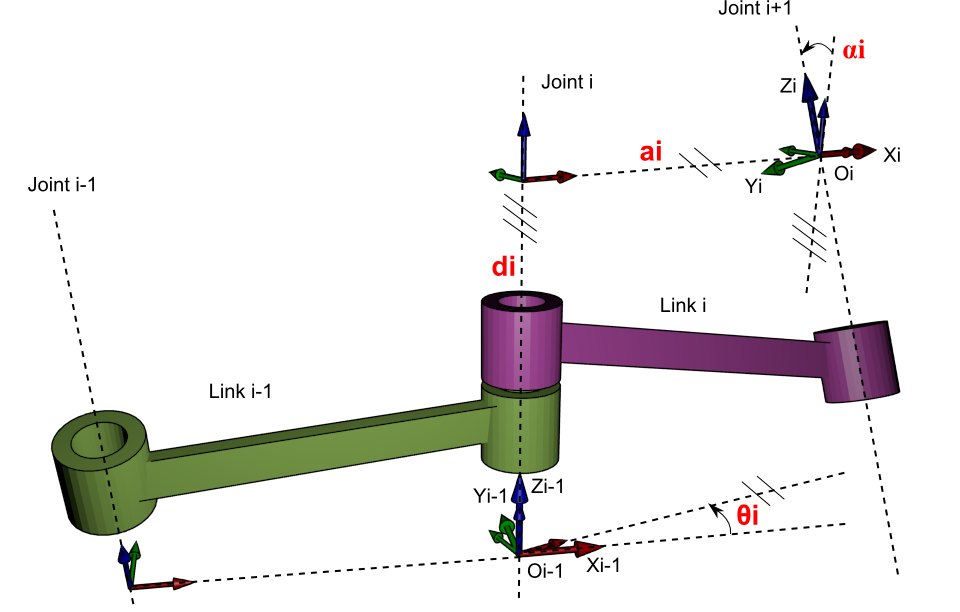
\includegraphics[width=0.95\textwidth]{imagens/dh.png}
    \caption{Minha primeira figura.}
    \label{fig:Figura1}
\end{figure}

\begin{equation}
M_{i,k}= M_{i,j} M_{j,k}
\end{equation}
% 
\begin{raggedright}
\bibliographystyle{plainnat}
\renewcommand{\bibsection}{
\chapter*{\begin{flushright}Referências bibliográficas\end{flushright}}
\addcontentsline{toc}{chapter}{Referências bibliográficas}
}
\lhead{REFERÊNCIAS BIBLIOGRÁFICAS}
\bibliography{referencias}
\newpage\lhead{\rightmark}
\end{raggedright}

% \chapter*{}
% \vfill
% \singlespacing
% \thispagestyle{empty}
% \begin{center}
% Este trabalho foi redigido em {\large\LaTeX}\ utilizando uma modifição do estilo \textsf{IC-UFAL}.
% As referências bibliográficas foram preparadas no \textsf{JabRef} e administradas pelo {\large\BibTeX}\ com o estilo \textsf{plainnat}.
% O texto utiliza fonte \NomeFonte em corpo de 12 pontos.
% A numeração dos capítulos segue com a familia tipográfica \NomeFonteCap.\\ 
% \vspace{.5cm}
% %\includegraphics[width=.5\textwidth]{Eye_of_Horus_bw}
% \end{center}

\end{document}
